\section[Cohomology of unitarizable modules for SO*(8)]{Cohomology for $\mathrm{SO}^*(8)$}

\subsection[so(8): (0, 1, 0, -6)]{$\boldsymbol{\mathfrak{s0}^*(8)\!:\; \omega_{2} - 6\omega_{4} }$}

Cone of unitarizable weights: $a_1\omega_1 + \left(a_{2} + 1\right)\omega_{2}+ a_3\omega_3  - \left(a_{1} + 2 \, a_{2} + a_{3} + 6\right)\omega_{4}$ \\


\begin{figure}[H]
  \centering
      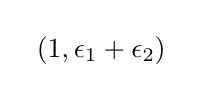
\begin{tikzpicture}[>=latex,line join=bevel,]
%%
\node (node_0) at (27.0bp,8.5bp) [draw,draw=none] {$(1, \epsilon_{1} + \epsilon_{2})$};
%
\end{tikzpicture}
  \caption{Nonnegative scalar products with noncompact roots}
\end{figure}
    

%\noindent $\lambda = $ $\left(a_{2} + 1\right)\omega_{2} - \left(a_{1} + 2 \, a_{2} + a_{3} + 6\right)\omega_{4}$ \\
\noindent Set of singular roots: $\emptyset$ \\

\begin{figure}[H]
  \centering
  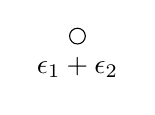
\begin{tikzpicture}
\draw[fill=white] (0 cm, 0 cm) circle (.1cm) node[below=4pt]{$\epsilon_{1} + \epsilon_{2}$};
\end{tikzpicture}
  \caption{The reduced Hermitian symmetric pair $(\mathfrak{g}_\lambda, \mathfrak{k}_\lambda)$}
\end{figure}

\begin{figure}[H]
  \centering
      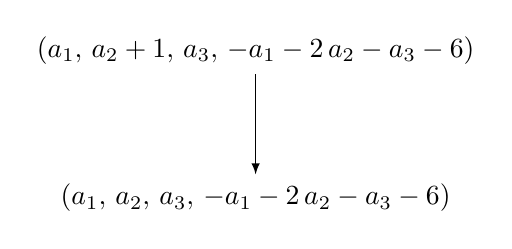
\begin{tikzpicture}[>=latex,line join=bevel,]
%%
\node (node_1) at (82.0bp,8.5bp) [draw,draw=none] {$\left(a_{1},\,a_{2},\,a_{3},\,-a_{1} - 2 \, a_{2} - a_{3} - 6\right)$};
  \node (node_0) at (82.0bp,61.5bp) [draw,draw=none] {$\left(a_{1},\,a_{2} + 1,\,a_{3},\,-a_{1} - 2 \, a_{2} - a_{3} - 6\right)$};
  \draw [black,->] (node_0) ..controls (82.0bp,23.805bp) and (82.0bp,34.034bp)  .. (node_1);
%
\end{tikzpicture}
  \caption{Nilpotent cohomology / BGG resolution}
\end{figure}

\subsection[so(8): (0, 0, 1, -3)]{$\boldsymbol{\mathfrak{s0}^*(8)\!:\; \omega_{3} - 3\omega_{4} }$}

Cone of unitarizable weights: $\left(a_{3} + 1\right)\omega_{3} - \left(a_{3} + 3\right)\omega_{4}$ \\

\begin{figure}[H]
  \centering
      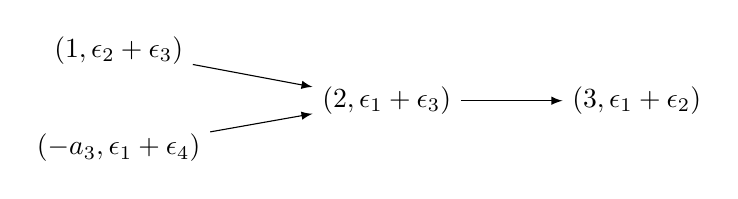
\begin{tikzpicture}[>=latex,line join=bevel,]
%%
\node (node_3) at (33.5bp,8.5bp) [draw,draw=none] {$(-a_{3}, \epsilon_{1} + \epsilon_{4})$};
  \node (node_2) at (220.0bp,25.5bp) [draw,draw=none] {$(3, \epsilon_{1} + \epsilon_{2})$};
  \node (node_1) at (130.0bp,25.5bp) [draw,draw=none] {$(2, \epsilon_{1} + \epsilon_{3})$};
  \node (node_0) at (33.5bp,43.5bp) [draw,draw=none] {$(1, \epsilon_{2} + \epsilon_{3})$};
  \draw [black,->] (node_0) ..controls (70.509bp,36.641bp) and (82.02bp,34.449bp)  .. (node_1);
  \draw [black,->] (node_3) ..controls (75.372bp,15.853bp) and (84.404bp,17.478bp)  .. (node_1);
  \draw [black,->] (node_1) ..controls (165.39bp,25.5bp) and (174.31bp,25.5bp)  .. (node_2);
%
\end{tikzpicture}
  \caption{Nonnegative scalar products with noncompact roots}
\end{figure}    

\noindent $\lambda = \omega_{3} -  3\omega_{4}$ \\
\noindent Set of singular roots: $\{\epsilon_{1} + \epsilon_{4}$\} \\

\begin{figure}[H]
  \centering
  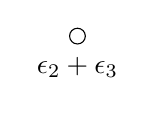
\begin{tikzpicture}
\draw[fill=white] (0 cm, 0 cm) circle (.1cm) node[below=4pt]{$\epsilon_{2} + \epsilon_{3}$};
\end{tikzpicture}
  \caption{The reduced Hermitian symmetric pair $(\mathfrak{g}_\lambda, \mathfrak{k}_\lambda)$}
\end{figure}

\begin{figure}[H]
  \centering
      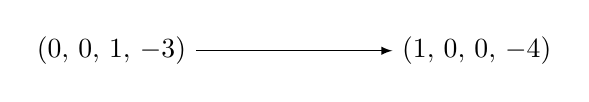
\begin{tikzpicture}[>=latex,line join=bevel,]
%%
\node (node_1) at (52.0bp,8.5bp) [draw,draw=none] {$\left(0,\,0,\,1,\,- 3\right)$};
  \node (node_0) at (183.5bp,8.5bp) [draw,draw=none] {$\left(1,\,0,\,0,\,- 4\right)$};
  \draw [black,->] (node_1) ..controls (112.53bp,8.5bp) and (121.18bp,8.5bp)  .. (node_0);
%
\end{tikzpicture}
  \caption{Nilpotent cohomology / BGG resolution}
\end{figure}

\noindent $\lambda = \left(a_{3} + 1\right)\omega_{3} - \left(a_{3} + 3\right)\omega_{4}$, $a_3 \geq 1$ \\
\noindent Set of singular roots: $\emptyset$ \\

\begin{figure}[H]
  \centering
  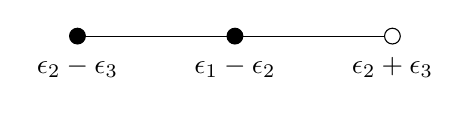
\begin{tikzpicture}
\draw (0 cm,0) -- (4 cm,0);
\draw[fill=black] (0 cm, 0 cm) circle (.1cm) node[below=4pt]{$\epsilon_{2} - \epsilon_{3}$};
\draw[fill=black] (2 cm, 0 cm) circle (.1cm) node[below=4pt]{$\epsilon_{1} - \epsilon_{2}$};
\draw[fill=white] (4 cm, 0 cm) circle (.1cm) node[below=4pt]{$\epsilon_{2} + \epsilon_{3}$};
\end{tikzpicture}
  \caption{The reduced Hermitian symmetric pair $(\mathfrak{g}_\lambda, \mathfrak{k}_\lambda)$}
\end{figure}

\begin{figure}[H]
  \centering
      \begin{tikzpicture}[>=latex,line join=bevel,]

 \node (node_0) at (0,3) [draw,draw=none] {$\left(0,\,0,\,a_{3} + 1,\,-a_{3} - 3\right)$};
 \node (node_1) at (3,2) [draw,draw=none] {$\left(1,\,0,\,a_{3},\,-a_{3} - 4\right)$};
 \node (node_2) at (6,1) [draw,draw=none] {$\left(0,\,1,\,a_{3} - 1,\,-a_{3} - 5\right)$};
 \node (node_3) at (9,0) [draw,draw=none] {$\left(0,\,0,\,a_{3} - 1,\,-a_{3} - 5\right)$};
 
  \draw [black,->] (node_0) edge (node_1);
  \draw [black,->] (node_1) edge (node_2);
  \draw [black,->] (node_2) edge (node_3);      
\end{tikzpicture}
  \caption{Nilpotent cohomology / BGG resolution}
\end{figure}

\subsection[so(8): (0, 0, 0, 0)]{$\boldsymbol{\mathfrak{s0}^*(8)\!:\; 0 }$}

Cone of unitarizable weights: $0$ \\


\begin{figure}[H]
  \centering
      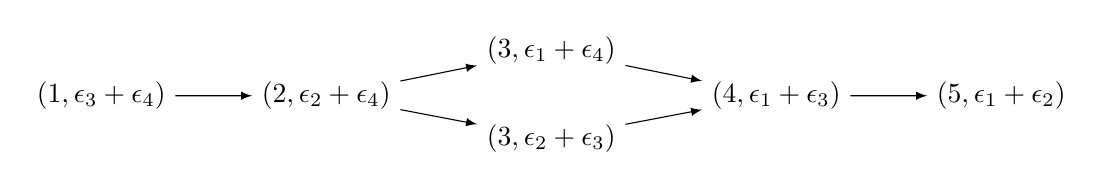
\begin{tikzpicture}[>=latex,line join=bevel,scale=0.9]
%%
\node (node_5) at (207.0bp,8.5bp) [draw,draw=none] {$(3, \epsilon_{2} + \epsilon_{3})$};
  \node (node_4) at (207.0bp,43.5bp) [draw,draw=none] {$(3, \epsilon_{1} + \epsilon_{4})$};
  \node (node_3) at (27.0bp,25.5bp) [draw,draw=none] {$(1, \epsilon_{3} + \epsilon_{4})$};
  \node (node_2) at (387.0bp,25.5bp) [draw,draw=none] {$(5, \epsilon_{1} + \epsilon_{2})$};
  \node (node_1) at (117.0bp,25.5bp) [draw,draw=none] {$(2, \epsilon_{2} + \epsilon_{4})$};
  \node (node_0) at (297.0bp,25.5bp) [draw,draw=none] {$(4, \epsilon_{1} + \epsilon_{3})$};
  \draw [black,->] (node_1) ..controls (152.48bp,32.553bp) and (161.51bp,34.399bp)  .. (node_4);
  \draw [black,->] (node_0) ..controls (332.39bp,25.5bp) and (341.31bp,25.5bp)  .. (node_2);
  \draw [black,->] (node_3) ..controls (62.393bp,25.5bp) and (71.311bp,25.5bp)  .. (node_1);
  \draw [black,->] (node_5) ..controls (242.39bp,15.144bp) and (251.31bp,16.867bp)  .. (node_0);
  \draw [black,->] (node_1) ..controls (152.39bp,18.856bp) and (161.31bp,17.133bp)  .. (node_5);
  \draw [black,->] (node_4) ..controls (242.48bp,36.447bp) and (251.51bp,34.601bp)  .. (node_0);
%
\end{tikzpicture}
  \caption{Nonnegative scalar products with noncompact roots}
\end{figure}
    

%\noindent $\lambda = $ $0$ \\
\noindent Set of singular roots: $\emptyset$ \\

\begin{figure}[H]
  \centering
  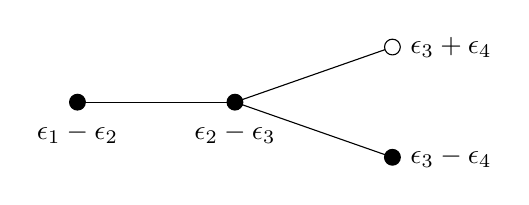
\begin{tikzpicture}
\draw (0 cm,0) -- (2 cm,0);
\draw (2 cm,0) -- (4 cm,0.7 cm);
\draw (2 cm,0) -- (4 cm,-0.7 cm);
\draw[fill=black] (0 cm, 0 cm) circle (.1cm) node[below=4pt]{$\epsilon_{1} - \epsilon_{2}$};
\draw[fill=black] (2 cm, 0 cm) circle (.1cm) node[below=4pt]{$\epsilon_{2} - \epsilon_{3}$};
\draw[fill=white] (4 cm, 0.7 cm) circle (.1cm) node[right=3pt]{$\epsilon_{3} + \epsilon_{4}$};
\draw[fill=black] (4 cm, -0.7 cm) circle (.1cm) node[right=3pt]{$\epsilon_{3} - \epsilon_{4}$};
\end{tikzpicture}
  \caption{The reduced Hermitian symmetric pair $(\mathfrak{g}_\lambda, \mathfrak{k}_\lambda)$}
\end{figure}

\begin{figure}[H]
  \centering
      \begin{tikzpicture}[>=latex,line join=bevel]
%%
\node (node_7) at (129.0bp,605.5bp) [draw,draw=none,scale=0.9] {$ \begin{tikzpicture}\draw (0 cm,0) -- (1.5 cm,0);\draw (1.5 cm,0) -- (3.0 cm,0.7 cm);\draw (1.5 cm,0) -- (3.0 cm,-0.7 cm);\draw[fill=black] (0.00 cm, 0 cm) circle (.1cm) node[below=4pt]{$0$};\draw[fill=black] (1.5 cm, 0 cm) circle (.1cm) node[below=4pt]{$0$};\draw[fill=white] (3.0 cm, 0.7 cm) circle (.1cm) node[right=3pt]{$0$};\draw[fill=black] (3.0 cm, -0.7 cm) circle (.1cm) node[right=3pt]{$0$};\end{tikzpicture} $};
  \node (node_6) at (129.0bp,510.0bp) [draw,draw=none,scale=0.9] {$ 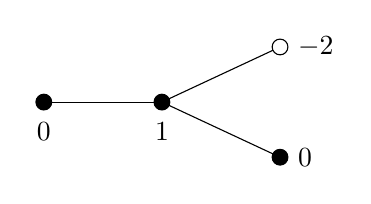
\begin{tikzpicture}\draw (0 cm,0) -- (1.5 cm,0);\draw (1.5 cm,0) -- (3.0 cm,0.7 cm);\draw (1.5 cm,0) -- (3.0 cm,-0.7 cm);\draw[fill=black] (0.00 cm, 0 cm) circle (.1cm) node[below=4pt]{$0$};\draw[fill=black] (1.5 cm, 0 cm) circle (.1cm) node[below=4pt]{$1$};\draw[fill=white] (3.0 cm, 0.7 cm) circle (.1cm) node[right=3pt]{$-2$};\draw[fill=black] (3.0 cm, -0.7 cm) circle (.1cm) node[right=3pt]{$0$};\end{tikzpicture} $};
  \node (node_5) at (198.0bp,318.0bp) [draw,draw=none,scale=0.9] {$ 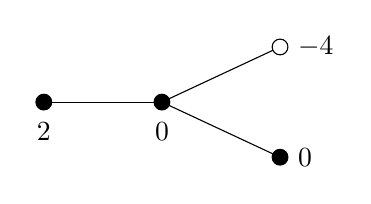
\begin{tikzpicture}\draw (0 cm,0) -- (1.5 cm,0);\draw (1.5 cm,0) -- (3.0 cm,0.7 cm);\draw (1.5 cm,0) -- (3.0 cm,-0.7 cm);\draw[fill=black] (0.00 cm, 0 cm) circle (.1cm) node[below=4pt]{$2$};\draw[fill=black] (1.5 cm, 0 cm) circle (.1cm) node[below=4pt]{$0$};\draw[fill=white] (3.0 cm, 0.7 cm) circle (.1cm) node[right=3pt]{$-4$};\draw[fill=black] (3.0 cm, -0.7 cm) circle (.1cm) node[right=3pt]{$0$};\end{tikzpicture} $};
  \node (node_4) at (129.0bp,30.0bp) [draw,draw=none,scale=0.9] {$ 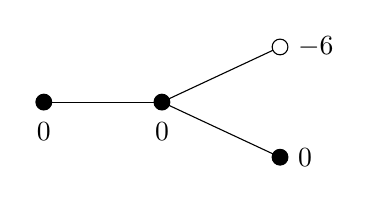
\begin{tikzpicture}\draw (0 cm,0) -- (1.5 cm,0);\draw (1.5 cm,0) -- (3.0 cm,0.7 cm);\draw (1.5 cm,0) -- (3.0 cm,-0.7 cm);\draw[fill=black] (0.00 cm, 0 cm) circle (.1cm) node[below=4pt]{$0$};\draw[fill=black] (1.5 cm, 0 cm) circle (.1cm) node[below=4pt]{$0$};\draw[fill=white] (3.0 cm, 0.7 cm) circle (.1cm) node[right=3pt]{$-6$};\draw[fill=black] (3.0 cm, -0.7 cm) circle (.1cm) node[right=3pt]{$0$};\end{tikzpicture} $};
  \node (node_3) at (129.0bp,222.0bp) [draw,draw=none,scale=0.9] {$ 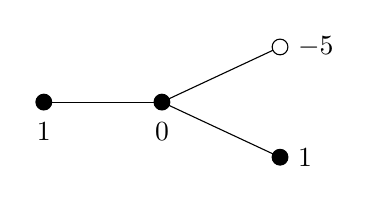
\begin{tikzpicture}\draw (0 cm,0) -- (1.5 cm,0);\draw (1.5 cm,0) -- (3.0 cm,0.7 cm);\draw (1.5 cm,0) -- (3.0 cm,-0.7 cm);\draw[fill=black] (0.00 cm, 0 cm) circle (.1cm) node[below=4pt]{$1$};\draw[fill=black] (1.5 cm, 0 cm) circle (.1cm) node[below=4pt]{$0$};\draw[fill=white] (3.0 cm, 0.7 cm) circle (.1cm) node[right=3pt]{$-5$};\draw[fill=black] (3.0 cm, -0.7 cm) circle (.1cm) node[right=3pt]{$1$};\end{tikzpicture} $};
  \node (node_2) at (129.0bp,126.0bp) [draw,draw=none,scale=0.9] {$ 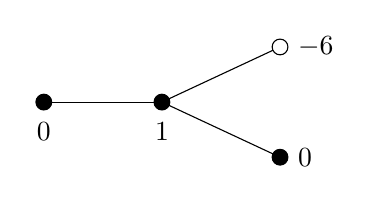
\begin{tikzpicture}\draw (0 cm,0) -- (1.5 cm,0);\draw (1.5 cm,0) -- (3.0 cm,0.7 cm);\draw (1.5 cm,0) -- (3.0 cm,-0.7 cm);\draw[fill=black] (0.00 cm, 0 cm) circle (.1cm) node[below=4pt]{$0$};\draw[fill=black] (1.5 cm, 0 cm) circle (.1cm) node[below=4pt]{$1$};\draw[fill=white] (3.0 cm, 0.7 cm) circle (.1cm) node[right=3pt]{$-6$};\draw[fill=black] (3.0 cm, -0.7 cm) circle (.1cm) node[right=3pt]{$0$};\end{tikzpicture} $};
  \node (node_1) at (60.0bp,318.0bp) [draw,draw=none,scale=0.9] {$ 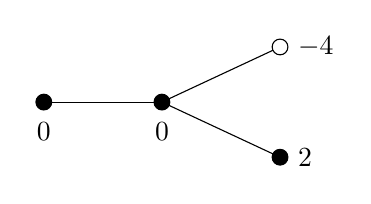
\begin{tikzpicture}\draw (0 cm,0) -- (1.5 cm,0);\draw (1.5 cm,0) -- (3.0 cm,0.7 cm);\draw (1.5 cm,0) -- (3.0 cm,-0.7 cm);\draw[fill=black] (0.00 cm, 0 cm) circle (.1cm) node[below=4pt]{$0$};\draw[fill=black] (1.5 cm, 0 cm) circle (.1cm) node[below=4pt]{$0$};\draw[fill=white] (3.0 cm, 0.7 cm) circle (.1cm) node[right=3pt]{$-4$};\draw[fill=black] (3.0 cm, -0.7 cm) circle (.1cm) node[right=3pt]{$2$};\end{tikzpicture} $};
  \node (node_0) at (129.0bp,414.0bp) [draw,draw=none,scale=0.9] {$ 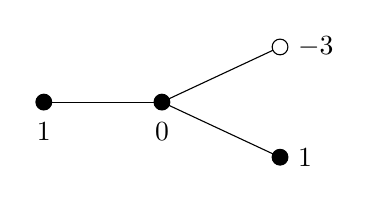
\begin{tikzpicture}\draw (0 cm,0) -- (1.5 cm,0);\draw (1.5 cm,0) -- (3.0 cm,0.7 cm);\draw (1.5 cm,0) -- (3.0 cm,-0.7 cm);\draw[fill=black] (0.00 cm, 0 cm) circle (.1cm) node[below=4pt]{$1$};\draw[fill=black] (1.5 cm, 0 cm) circle (.1cm) node[below=4pt]{$0$};\draw[fill=white] (3.0 cm, 0.7 cm) circle (.1cm) node[right=3pt]{$-3$};\draw[fill=black] (3.0 cm, -0.7 cm) circle (.1cm) node[right=3pt]{$1$};\end{tikzpicture} $};
  \draw [black,->] (node_6) ..controls (129.0bp,471.73bp) and (129.0bp,462.87bp)  .. (node_0);
  \draw [black,->] (node_3) ..controls (129.0bp,183.73bp) and (129.0bp,174.87bp)  .. (node_2);
  \draw [black,->] (node_5) ..controls (170.19bp,279.11bp) and (163.13bp,269.5bp)  .. (node_3);
  \draw [black,->] (node_0) ..controls (156.81bp,375.11bp) and (163.87bp,365.5bp)  .. (node_5);
  \draw [black,->] (node_7) ..controls (129.0bp,567.84bp) and (129.0bp,558.89bp)  .. (node_6);
  \draw [black,->] (node_1) ..controls (87.814bp,279.11bp) and (94.869bp,269.5bp)  .. (node_3);
  \draw [black,->] (node_0) ..controls (101.19bp,375.11bp) and (94.131bp,365.5bp)  .. (node_1);
  \draw [black,->] (node_2) ..controls (129.0bp,87.727bp) and (129.0bp,78.866bp)  .. (node_4);
%
\end{tikzpicture}
  \caption{Nilpotent cohomology / BGG resolution}
\end{figure}

\subsection[so(8): (0, 0, 0, -2)]{$\boldsymbol{\mathfrak{s0}^*(8)\!:\; -2\omega_{4} }$}

Cone of unitarizable weights: $-2\omega_{4}$ \\


\begin{figure}[H]
  \centering
      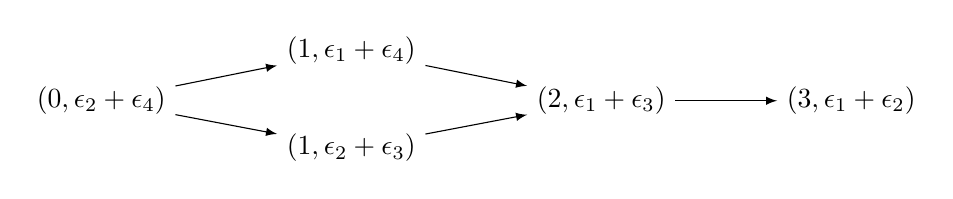
\begin{tikzpicture}[>=latex,line join=bevel,]
%%
\node (node_4) at (27.0bp,25.5bp) [draw,draw=none] {$(0, \epsilon_{2} + \epsilon_{4})$};
  \node (node_3) at (117.0bp,8.5bp) [draw,draw=none] {$(1, \epsilon_{2} + \epsilon_{3})$};
  \node (node_2) at (297.0bp,25.5bp) [draw,draw=none] {$(3, \epsilon_{1} + \epsilon_{2})$};
  \node (node_1) at (117.0bp,43.5bp) [draw,draw=none] {$(1, \epsilon_{1} + \epsilon_{4})$};
  \node (node_0) at (207.0bp,25.5bp) [draw,draw=none] {$(2, \epsilon_{1} + \epsilon_{3})$};
  \draw [black,->] (node_4) ..controls (62.393bp,18.856bp) and (71.311bp,17.133bp)  .. (node_3);
  \draw [black,->] (node_3) ..controls (152.39bp,15.144bp) and (161.31bp,16.867bp)  .. (node_0);
  \draw [black,->] (node_0) ..controls (242.39bp,25.5bp) and (251.31bp,25.5bp)  .. (node_2);
  \draw [black,->] (node_1) ..controls (152.48bp,36.447bp) and (161.51bp,34.601bp)  .. (node_0);
  \draw [black,->] (node_4) ..controls (62.481bp,32.553bp) and (71.507bp,34.399bp)  .. (node_1);
%
\end{tikzpicture}
  \caption{Nonnegative scalar products with noncompact roots}
\end{figure}
    

%\noindent $\lambda = $ $-2\omega_{4}$ \\
\noindent Set of singular roots: $\{\epsilon_{2} + \epsilon_{4}$\} \\

\begin{figure}[H]
  \centering
  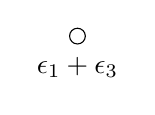
\begin{tikzpicture}
\draw[fill=white] (0 cm, 0 cm) circle (.1cm) node[below=4pt]{$\epsilon_{1} + \epsilon_{3}$};
\end{tikzpicture}
  \caption{The reduced Hermitian symmetric pair $(\mathfrak{g}_\lambda, \mathfrak{k}_\lambda)$}
\end{figure}

\begin{figure}[H]
  \centering
      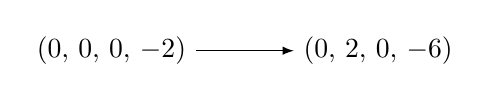
\begin{tikzpicture}[>=latex,line join=bevel,]
%%
\node (node_1) at (126.0bp,8.5bp) [draw,draw=none] {$\left(0,\,2,\,0,\,-6\right)$};
  \node (node_0) at (30.0bp,8.5bp) [draw,draw=none] {$\left(0,\,0,\,0,\,-2\right)$};
  \draw [black,->] (node_0) ..controls (68.273bp,8.5bp) and (77.134bp,8.5bp)  .. (node_1);
%
\end{tikzpicture}
  \caption{Nilpotent cohomology / BGG resolution}
\end{figure}

\subsection[so(8): (1, 1, 0, -7)]{$\boldsymbol{\mathfrak{s0}^*(8)\!:\; \omega_{1} + \omega_{2} - 7\omega_{4} }$}

Cone of unitarizable weights: $\left(a_{1} + 1\right)\omega_{1} + \left(a_{2} + 1\right)\omega_{2} + a_3\omega_3 -\left(a_{1} + 2 \, a_{2} + a_{3} + 7\right)\omega_{4}$ \\


\begin{figure}[H]
  \centering
      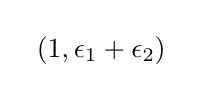
\begin{tikzpicture}[>=latex,line join=bevel,]
%%
\node (node_0) at (27.0bp,8.5bp) [draw,draw=none] {$(1, \epsilon_{1} + \epsilon_{2})$};
%
\end{tikzpicture}
  \caption{Nonnegative scalar products with noncompact roots}
\end{figure}
    

%\noindent $\lambda = $ $\left(a_{1} + 1\right)\omega_{1} + \left(a_{2} + 1\right)\omega_{2} - \left(a_{1} + 2 \, a_{2} + a_{3} + 7\right)\omega_{4}$ \\
\noindent Set of singular roots: $\emptyset$ \\

\begin{figure}[H]
  \centering
  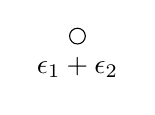
\begin{tikzpicture}
\draw[fill=white] (0 cm, 0 cm) circle (.1cm) node[below=4pt]{$\epsilon_{1} + \epsilon_{2}$};
\end{tikzpicture}
  \caption{The reduced Hermitian symmetric pair $(\mathfrak{g}_\lambda, \mathfrak{k}_\lambda)$}
\end{figure}

\begin{figure}[H]
  \centering
      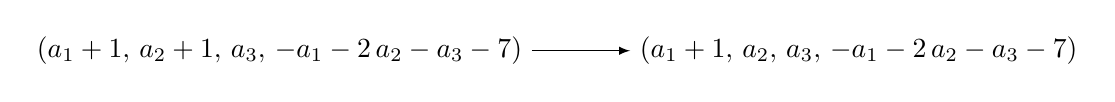
\begin{tikzpicture}[>=latex,line join=bevel,]
%%
\node (node_1) at (299.0bp,8.5bp) [draw,draw=none] {$\left(a_{1} + 1,\,a_{2},\,a_{3},\,-a_{1} - 2 \, a_{2} - a_{3} - 7\right)$};
  \node (node_0) at (90.5bp,8.5bp) [draw,draw=none] {$\left(a_{1} + 1,\,a_{2} + 1,\,a_{3},\,-a_{1} - 2 \, a_{2} - a_{3} - 7\right)$};
  \draw [black,->] (node_0) ..controls (189.61bp,8.5bp) and (198.17bp,8.5bp)  .. (node_1);
%
\end{tikzpicture}
  \caption{Nilpotent cohomology / BGG resolution}
\end{figure}

\subsection[so(8): (1, 0, 1, -5)]{$\boldsymbol{\mathfrak{s0}^*(8)\!:\; \omega_{1} + \omega_{3} - 5\omega_{4} }$}

Cone of unitarizable weights: $\left(a_{1} + 1\right)\omega_{1} + \left(a_{3} + 1\right)\omega_{3} - \left(a_{1} + a_{3} + 5\right)\omega_{4}$ \\


\begin{figure}[H]
  \centering
      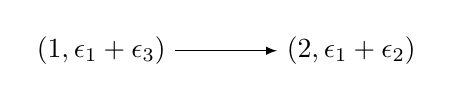
\begin{tikzpicture}[>=latex,line join=bevel,]
%%
\node (node_1) at (27.0bp,8.5bp) [draw,draw=none] {$(1, \epsilon_{1} + \epsilon_{3})$};
  \node (node_0) at (117.0bp,8.5bp) [draw,draw=none] {$(2, \epsilon_{1} + \epsilon_{2})$};
  \draw [black,->] (node_1) ..controls (62.393bp,8.5bp) and (71.311bp,8.5bp)  .. (node_0);
%
\end{tikzpicture}
  \caption{Nonnegative scalar products with noncompact roots}
\end{figure}
    

%\noindent $\lambda = $ $\left(a_{1} + 1\right)\omega_{1} + \left(a_{3} + 1\right)\omega_{3} - \left(a_{1} + a_{3} + 5\right)\omega_{4}$ \\
\noindent Set of singular roots: $\emptyset$ \\

\begin{figure}[H]
  \centering
  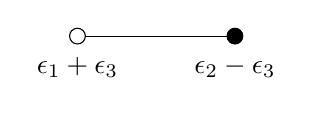
\begin{tikzpicture}
\draw (0 cm,0) -- (2 cm,0);
\draw[fill=white] (0 cm, 0 cm) circle (.1cm) node[below=4pt]{$\epsilon_{1} + \epsilon_{3}$};
\draw[fill=black] (2 cm, 0 cm) circle (.1cm) node[below=4pt]{$\epsilon_{2} - \epsilon_{3}$};
\end{tikzpicture}
  \caption{The reduced Hermitian symmetric pair $(\mathfrak{g}_\lambda, \mathfrak{k}_\lambda)$}
\end{figure}

\begin{figure}[H]
  \centering
      \begin{tikzpicture}[>=latex,line join=bevel,]


 \node (node_0) at (0,3) [draw,draw=none] {$\left(a_{1} + 1,\,0,\,a_{3} + 1,\,-a_{1} - a_{3} - 5\right)$};
 \node (node_1) at (3,2) [draw,draw=none] {$\left(a_{1},\,1,\,a_{3},\,-a_{1} - a_{3} - 6\right)$};
 \node (node_2) at (6,1) [draw,draw=none] {$\left(a_{1},\,0,\,a_{3},\,-a_{1} - a_{3} - 6\right)$};
 
  \draw [black,->] (node_0) edge (node_1);
  \draw [black,->] (node_1) edge (node_2);
      
\end{tikzpicture}
  \caption{Nilpotent cohomology / BGG resolution}
\end{figure}

\subsection[so(8): (1, 0, 0, -3)]{$\boldsymbol{\mathfrak{s0}^*(8)\!:\; \omega_{1} - 3\omega_{4} }$}

Cone of unitarizable weights: $\left(a_{1} + 1\right)\omega_{1} - \left(a_{1} + 3\right)\omega_{4}$ \\


\begin{figure}[H]
  \centering
      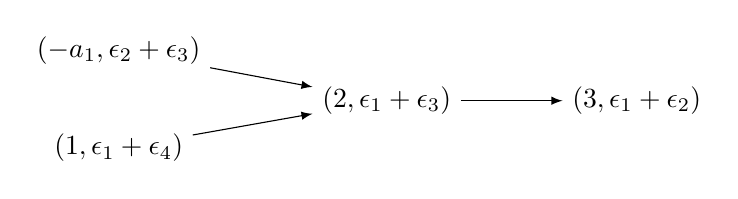
\begin{tikzpicture}[>=latex,line join=bevel,]
%%
\node (node_3) at (130.0bp,25.5bp) [draw,draw=none] {$(2, \epsilon_{1} + \epsilon_{3})$};
  \node (node_2) at (220.0bp,25.5bp) [draw,draw=none] {$(3, \epsilon_{1} + \epsilon_{2})$};
  \node (node_1) at (33.5bp,43.5bp) [draw,draw=none] {$(-a_{1}, \epsilon_{2} + \epsilon_{3})$};
  \node (node_0) at (33.5bp,8.5bp) [draw,draw=none] {$(1, \epsilon_{1} + \epsilon_{4})$};
  \draw [black,->] (node_3) ..controls (165.39bp,25.5bp) and (174.31bp,25.5bp)  .. (node_2);
  \draw [black,->] (node_1) ..controls (75.372bp,35.715bp) and (84.404bp,33.994bp)  .. (node_3);
  \draw [black,->] (node_0) ..controls (70.509bp,14.978bp) and (82.02bp,17.049bp)  .. (node_3);
%
\end{tikzpicture}
  \caption{Nonnegative scalar products with noncompact roots}
\end{figure}
    

\noindent $\lambda =\omega_{1} - 3\omega_{4}$ \\
\noindent Set of singular roots: $\{\epsilon_{2} + \epsilon_{3}$\} \\

\begin{figure}[H]
  \centering
  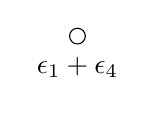
\begin{tikzpicture}
\draw[fill=white] (0 cm, 0 cm) circle (.1cm) node[below=4pt]{$\epsilon_{1} + \epsilon_{4}$};
\end{tikzpicture}
  \caption{The reduced Hermitian symmetric pair $(\mathfrak{g}_\lambda, \mathfrak{k}_\lambda)$}
\end{figure}

\begin{figure}[H]
  \centering
      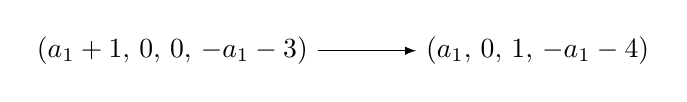
\begin{tikzpicture}[>=latex,line join=bevel,]
%%
\node (node_1) at (183.5bp,8.5bp) [draw,draw=none] {$\left(a_{1},\,0,\,1,\,-a_{1} - 4\right)$};
  \node (node_0) at (52.0bp,8.5bp) [draw,draw=none] {$\left(a_{1} + 1,\,0,\,0,\,-a_{1} - 3\right)$};
  \draw [black,->] (node_0) ..controls (112.53bp,8.5bp) and (121.18bp,8.5bp)  .. (node_1);
%
\end{tikzpicture}
  \caption{Nilpotent cohomology / BGG resolution}
\end{figure}

\noindent $\lambda = $ $\left(a_{1} + 1\right)\omega_{1} - \left(a_{1} + 3\right)\omega_{4}$, $a_1 \geq 1$ \\
\noindent Set of singular roots: $\emptyset$ \\

\begin{figure}[H]
  \centering
  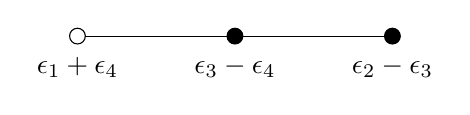
\begin{tikzpicture}
\draw (0 cm,0) -- (4 cm,0);
\draw[fill=white] (0 cm, 0 cm) circle (.1cm) node[below=4pt]{$\epsilon_{1} + \epsilon_{4}$};
\draw[fill=black] (2 cm, 0 cm) circle (.1cm) node[below=4pt]{$\epsilon_{3} - \epsilon_{4}$};
\draw[fill=black] (4 cm, 0 cm) circle (.1cm) node[below=4pt]{$\epsilon_{2} - \epsilon_{3}$};
\end{tikzpicture}
  \caption{The reduced Hermitian symmetric pair $(\mathfrak{g}_\lambda, \mathfrak{k}_\lambda)$}
\end{figure}

\begin{figure}[H]
  \centering
      \begin{tikzpicture}[>=latex,line join=bevel,]


 \node (node_0) at (0,3) [draw,draw=none] {$\left(a_{1} + 1,\,0,\,0,\,-a_{1} - 3\right)$};
 \node (node_1) at (3,2) [draw,draw=none] {$\left(a_{1},\,0,\,1,\,-a_{1} - 4\right)$};
 \node (node_2) at (6,1) [draw,draw=none] {$\left(a_{1} - 1,\,1,\,0,\,-a_{1} - 5\right)$};
 \node (node_3) at (9,0) [draw,draw=none] {$\left(a_{1} - 1,\,0,\,0,\,-a_{1} - 5\right)$};
 
  \draw [black,->] (node_0) edge (node_1);
  \draw [black,->] (node_1) edge (node_2);
  \draw [black,->] (node_2) edge (node_3);         
 
\end{tikzpicture}
  \caption{Nilpotent cohomology / BGG resolution}
\end{figure}